\chapter{An Introduction to Fourier Transforms}\label{fourier_transform_basics}\noindent
Fourier transforms are used extensively in the subject of diffraction and
imaging, so in this chapter we present a basic introduction describing the
Fourier transform and its most commonly used properties. These properties will
be fundamental for both for the description scattering and for the explanation
of image reconstruction algorithms.

\section{Continuous Fourier Transform}

We will start by defining the continuous forward Fourier transform, following crystallographic tradition, as,
\begin{equation}
\hat{f}(q) = \mathscr{F}f = \int \limits_{-\infty}^{\infty} 
f(x) \exp(2 \pi i q \cdot x) \, dx
\end{equation}
and the inverse transform as,
\begin{equation}
f(x) = \mathscr{F}^{-1}\hat{f} = \int \limits_{-\infty}^{\infty} 
\hat{f}(q) \exp(-2 \pi i q \cdot x) \, dq.
\end{equation}
The following properties of the Fourier transform will be important for the rest of the thesis:
%The Fourier transform has the following properties:
\begin{enumerate}
\item The Fourier transform is a linear transformation. For any two complex
  numbers $a$ and $b$,
\begin{equation}
\mathscr{F}\left\{ a f(x) + b g(x)\right\} = a \mathscr{F}f(x) + b \mathscr{F}g(x)
\end{equation}

\item The Fourier transform of a real function $f(x)$ is a hermitian function,  
\begin{equation}
\hat{f}(q) = \overline{\hat{f}(-q)}
\end{equation}
where $\overline{x}$ represents the complex conjugate of $x$.
\item The Fourier transform of an hermitian function $f(x)$ is a real function,
\begin{equation}
Im\left[\hat{f}(q)\right] = 0
\end{equation}
where $Im\left[x\right]$ represents the imaginary part of $x$.
\item The Fourier transform of a function translated by an amount $\Delta x$ is
  related to the transform of the original function by a factor of $\exp(2 \pi i
  \Delta x q)$ ,
  \begin{equation}
    \mathscr{F} f(x+\Delta x) = \exp(2 \pi i \Delta x q) \mathscr{F} f(x)
\end{equation}

\item The integral of the square of the absolute value of a function and it's Fourier transform are identical
\begin{equation}
\int |\hat{f}(q)|^2 dq = \int |f(x)|^2 dx.
\end{equation}
This is usually as Parseval's theorem or Rayleigh's energy theorem

\item The convolution of any two functions is equal to the inverse Fourier transform of the product of the forward Fourier transform of those two functions,
\begin{eqnarray}
f(x) * g(x) & = & \int f(\tau) g(x-\tau) \, d\tau \nonumber \\
& = & \mathscr{F}^{-1}\left\{\mathscr{F}f(x) \times \mathscr{F}g(x)\right\}
\end{eqnarray}
where $f(x) * g(x)$ denotes the convolution of $f(x)$ with $g(x)$. This property
is known as the convolution theorem.

\item The cross-correlation of any two functions is equal to the inverse Fourier
  transform of the product of the forward Fourier transform of one function with
  the complex conjugate of the forward Fourier transform the other function,
\begin{eqnarray}
f(x) \star g(x) & = & \int f(\tau) g(x+\tau) \, d\tau \nonumber \\ 
& = & \mathscr{F}^{-1}\left\{\mathscr{F}f(x) \times \overline{\mathscr{F}g(x)}\right\}
\end{eqnarray}
where $f(x) \star g(x)$ denotes the cross-correlation of $f(x)$ with $g(x)$.
 
\item Finally the correlation of a function with itself, also known as
  autocorrelation is equal to the inverse Fourier transform of the absolute
  value squared of the forward Fourier transform of that function,
  \begin{eqnarray}
f(x) \star f(x) & = & \mathscr{F}^{-1}\left\{\mathscr{F}f(x) 
  \times \overline{\mathscr{F}f(x)}\right\} \nonumber \\
& = & \mathscr{F}^{-1}\left\{|\mathscr{F}f(x)|^2\right\}
\end{eqnarray}
\end{enumerate}

\section{Discrete Fourier Transform}

In practise we will be dealing with signals which are not continuous, but
discrete, as most signal recording is done digitally nowadays and to be able to
performe numerical computations with any input we first need to digitize
it. Fortunately there is a discrete analogue of the Fourier transform called
the discrete Fourier transform (DFT). The one dimensional discrete Fourier
transform of a vector $\mathbf x$ of length N is defined by
\begin{equation}
\hat{\mathbf x}_k = \mathscr{F}\left\{ \mathbf x\right\}_k = \frac{1}{\sqrt{N}} \sum
\limits_{n=0}^{N} \mathbf x_n \exp\left(2 \pi i k \frac{n}{N}\right) \, ,
\end{equation}
and the inverse pair as
\begin{equation}
{\mathbf x}_n = \mathscr{F}^{-1}\left\{ \mathbf x\right\}_n = \frac{1}{\sqrt{M}} \sum
\limits_{k=0}^{M} \hat{\mathbf x}_k \exp\left(-2 \pi i n \frac{k}{M}\right) \, .
\end{equation}

Throughout this thesis we will commit a slight abuse of notation and use
$\mathscr{F}$ to symbolize both the continuous Fourier transform, when the
operand is a function, and the discrete Fourier transform, when the operand is a
vector.
 
The DFT has properties analogous to most properties of its continuous
counterpart, in particular it's a distance preserving transform, that is the distance between two vectors is the same before and after transformation
\begin{equation}
  |\mathscr{F}(x)-\mathscr{F}(y)| = |(x-y)|
\end{equation}
which follows from both the linearity of the transform and Parseval's theorem.
It also also fulfills the convolution theorem if we define the discrete
convolution as
\begin{equation}
  (\mathbf a * \mathbf b)_n = \sum \limits_{m = 0}^{N-1} \mathbf a_m 
  \mathbf  b_{n-m \bmod N} .
\end{equation}
Notice the modulus $N$ in the index of $b$. This detail will lead to important
consequences.

\section{Sampling and oversampling}


An arbitrary bandlimited signal $f(x)$ with bandwidth $2B$, meaning a signal which has
$\hat{f}(x) = 0$ for every $|x| > B$, can be perfectly reconstructed from
the same signal sampled in steps of length smaller or equal to $1/2B$. $2B$ is
known as the {\em Nyquist rate}. This derives from the fact that the continuous
Fourier transform of $f(x)$ can be exactly reconstructed equidistant samples
separated by a step $s < 1/2B$,
\begin{eqnarray}
rect_B(q) & = & 
\begin{cases}
  1  & \text{if $|q| \le B$,}\\
  0  & \text{if $q > B$.}
\end{cases}\\
\text{\Sha}_s(x) & = & \sum_{i = -\infty}^{\infty} \delta(x-i s)\\
\hat{f}(q) & = & \mathscr{F}\{\text{\Sha}_s(x) f(x)\} rect_B(q)
\end{eqnarray}
where $\delta(x)$ represents the Dirac delta function.

\begin{figure}[h!]
  \centering
  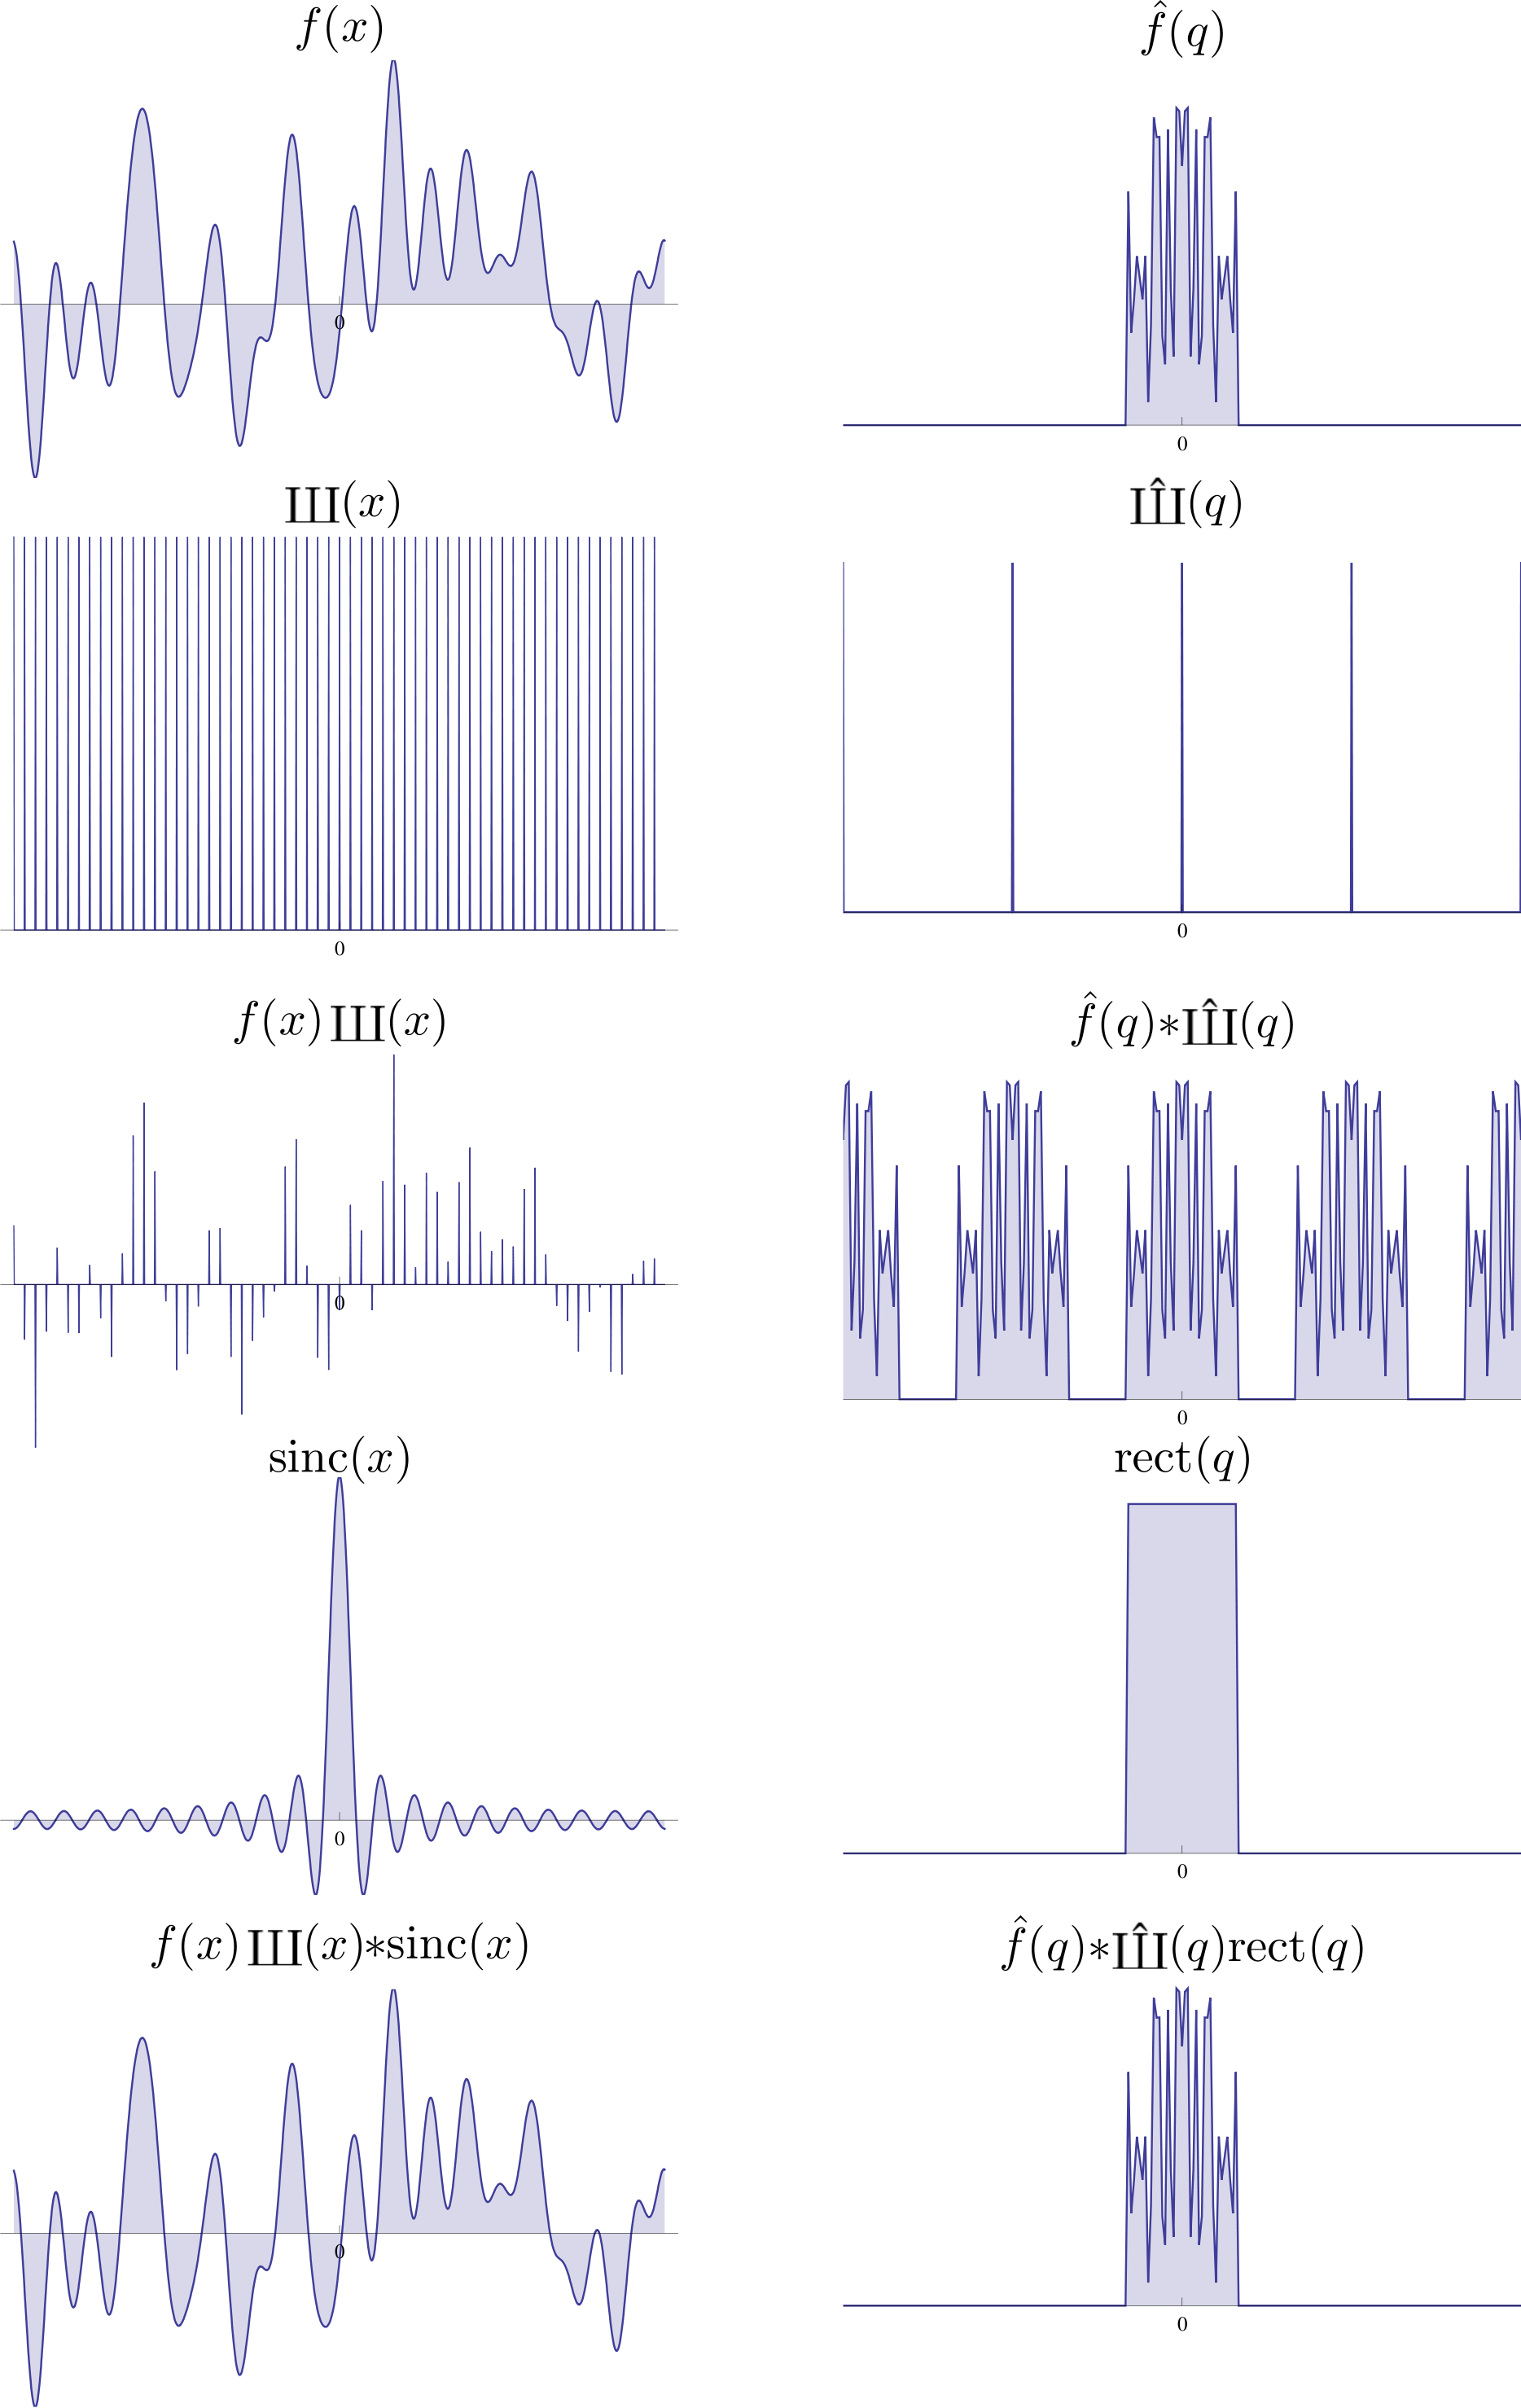
\includegraphics[width=0.7 \columnwidth]{Sampling2.png}
  \caption{Reconstruction of a bandlimited signal from discrete samples taken at
    a frequency higher than the Nyquist rate.}\
  \label{Fig_Sampling}
\end{figure}

As figure \ref{Fig_Sampling} shows sampling a signal causes its spectrum to be
replicated in Fourier space. The distance between the replicas is proportional
to the sampling frequency due to the scaling property of the Fourier
transform. If the sampling frequency is below the Nyquist rate the spectras will
overlap and a perfect reconstruct is no longer possible, a phenomenon known as
aliasing. We call such a sampled signal {\em undersampled}. If on the other hand
the sampling frequency is higher than the Nyquist rate we call it {\em
  oversampled} and we define {\em oversampling ratio}, $\sigma$, as the ratio between the
sampling frequency and the Nyquist rate, or equivalently the fraction between
the center of two replicas of the spectrum in Fourier space and the region for
which the spectrum is different than zero, as illustrated in figure \ref{Fig:OversamplingRatio}.

\begin{figure}[h]
  \centering
  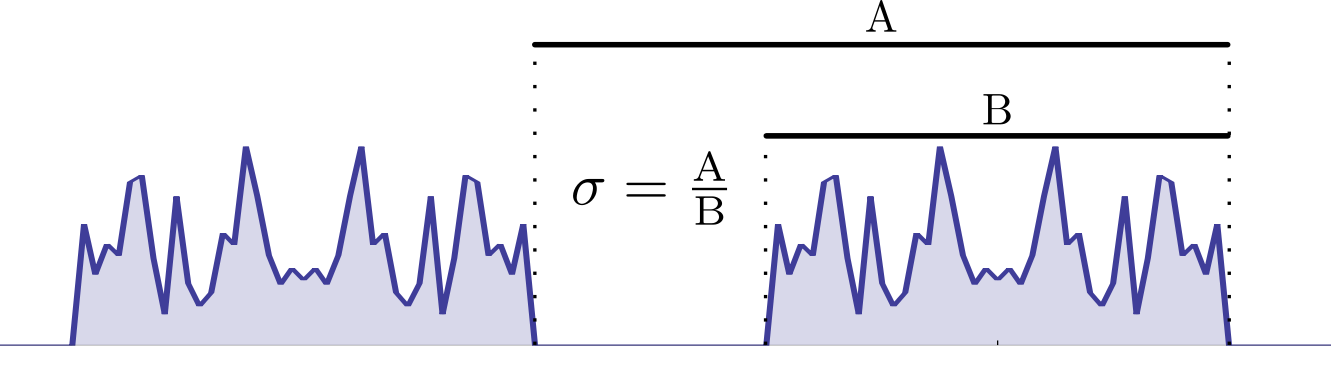
\includegraphics[width=0.8 \columnwidth]{Oversampling.png}
  \caption{The oversampling ratio, denoted by $\sigma$, is the ratio between the
    size of the Fourier space and the region used by the signal.}
  \label{Fig:OversamplingRatio}
\end{figure}